% -*- latex -*-
%%%%%%%%%%%%%%%%%%%%%%%%%%%%%%%%%%%%%%%%%%%%%%%%%%%%%%%%%%%%%%%%
%%%%%%%%%%%%%%%%%%%%%%%%%%%%%%%%%%%%%%%%%%%%%%%%%%%%%%%%%%%%%%%%
%%%%
%%%% This text file is part of the source of 
%%%% `Parallel Programming in MPI and OpenMP'
%%%% by Victor Eijkhout, copyright 2012-8
%%%%
%%%% mandelbrot.tex : a mandelbrot project
%%%%
%%%%%%%%%%%%%%%%%%%%%%%%%%%%%%%%%%%%%%%%%%%%%%%%%%%%%%%%%%%%%%%%
%%%%%%%%%%%%%%%%%%%%%%%%%%%%%%%%%%%%%%%%%%%%%%%%%%%%%%%%%%%%%%%%

If you've never heard the name \indexterm{Mandelbrot set}, you
probably recognize the picture; figure~\ref{fig:mandelbrotset}
%
\begin{figure}[ht]

\includegraphics{mandelbrot}
\label{fig:mandelbrotset}
\caption{The Mandelbrot set}
\end{figure}
%
Its formal definition is as follows:
\begin{quotation}\noindent
  A point $c$ in the complex plane is part of the Mandelbrot set if 
  the series $x_n$ defined by 
  \[ 
  \begin{cases}
    x_0=0\\ x_{n+1}=x_n^2+c
  \end{cases}
  \] satisfies \[ \forall_n\colon |x_n|\leq 2. \]  
\end{quotation}
It is easy to see that only points $c$ in the bounding circle
$|c|< 2$ qualify, but
apart from that it's hard to say much without a lot more thinking.
Or computing; and that's what we're going to do.

In this set of exercises you are going to take an example program
\n{mandel_main.cxx} and extend it to use a variety of MPI programming
constructs.  This program has been set up as a
\indexterm{manager-worker} model: there is one manager processor (for a
change this is the last processor, rather than zero) which gives out
work to, and accepts results from, the worker processors. It then
takes the results and constructs an image file from them.

\Level 0 {Invocation}

The \n{mandel_main} program is called as
\begin{verbatim}
mpirun -np 123 mandel_main steps 456 iters 789
\end{verbatim}
where the \n{steps} parameter indicates how many steps in $x,y$
direction there are in the image, and \n{iters} gives the maximum
number of iterations in the \n{belong} test.

If you forget the parameter, you can call the program with
\begin{verbatim}
mandel_serial -h
\end{verbatim}
and it will print out the usage information.

\Level 0 {Tools}

The driver part of the Mandelbrot program is simple. There is a 
circle object that can generate coordinates
\cverbatimsnippet{circledef}
and a global routine that tests whether a coordinate is in the set,
at least up to an iteration bound. It returns zero if the 
series from the given starting point has not diverged,
or the iteration number in which it diverged if it did so.
\cverbatimsnippet{belongs}
In the former case,  the point could be in the Mandelbrot set, 
and we colour it black, in the latter case we give it a colour
depending on the iteration number.
\cverbatimsnippet{pickcolour}
We use a fairly simple code for the worker processes: they 
execute a loop in which they wait 
for input, process it, return the result.
\cverbatimsnippet{waitforwork}

A very simple solution using blocking sends on the manager is given:
\cverbatimsnippet{serialaddtask}

\begin{exercise}
  Explain why this solution is very inefficient. Make a trace of its
  execution that bears this out.
\end{exercise}

\begin{figure}[ht]
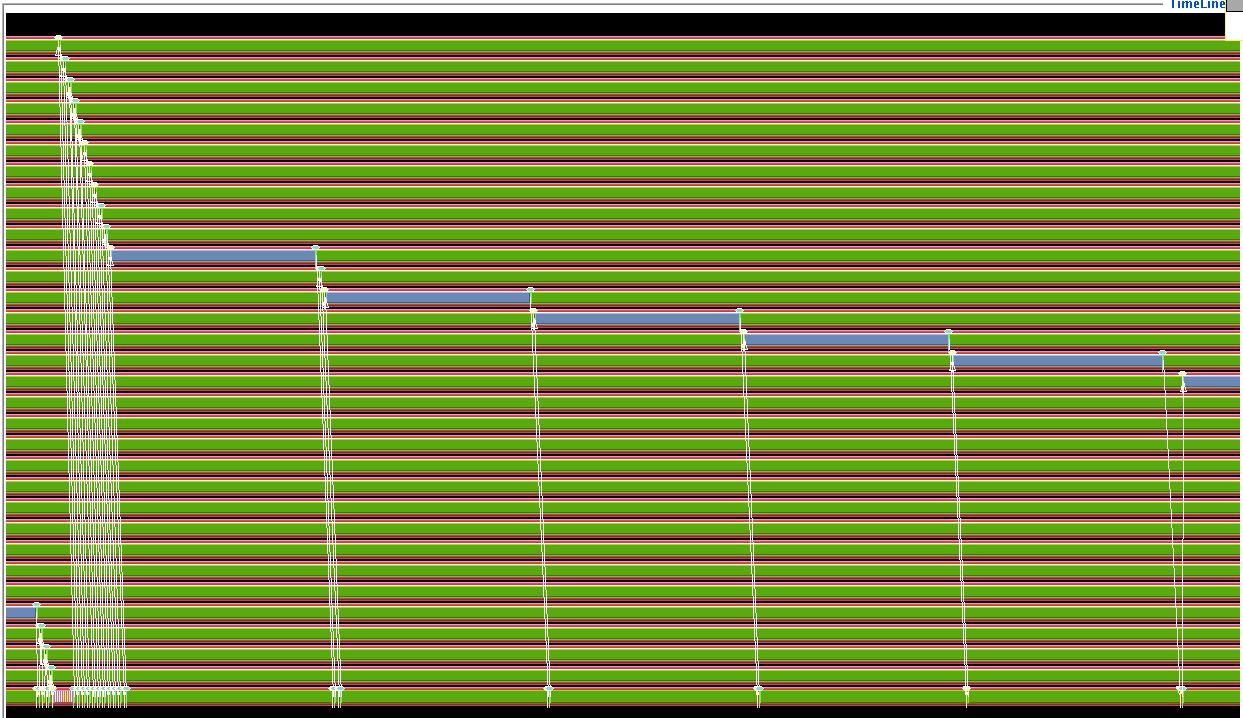
\includegraphics[scale=.35]{mandelserial}
\caption{Trace of a serial Mandelbrot calculation}
\label{fig:mandel-serial}
\end{figure}

\Level 0 {Bulk task scheduling}
\label{proj:mandel-bulk}

The previous section showed a very inefficient solution, but that was mostly
intended to set up the code base. If all tasks take about the same amount of time,
you can give each process a task, and then wait on them all to finish. A~first way
to do this is with non-blocking sends.

\begin{exercise}
  Code a  solution where you give a task to all worker processes
  using non-blocking sends and receives, and then wait for these tasks
  with \n{MPI_Waitall}
  to finish before you give a new round of data to all workers.
  Make a trace of the execution of this and report on the total time.

  You can do this by writing a new class that inherits from \n{queue},
  and that provides its own \n{addtask} method:
  \cverbatimsnippet{bulkq}
  You will also have to override the \n{complete} method: when the circle 
  object indicates that all coordinates have been generated, not all
  workers will be busy, so you need to supply the proper \n{MPI_Waitall}
  call.
\end{exercise}

\begin{figure}[ht]
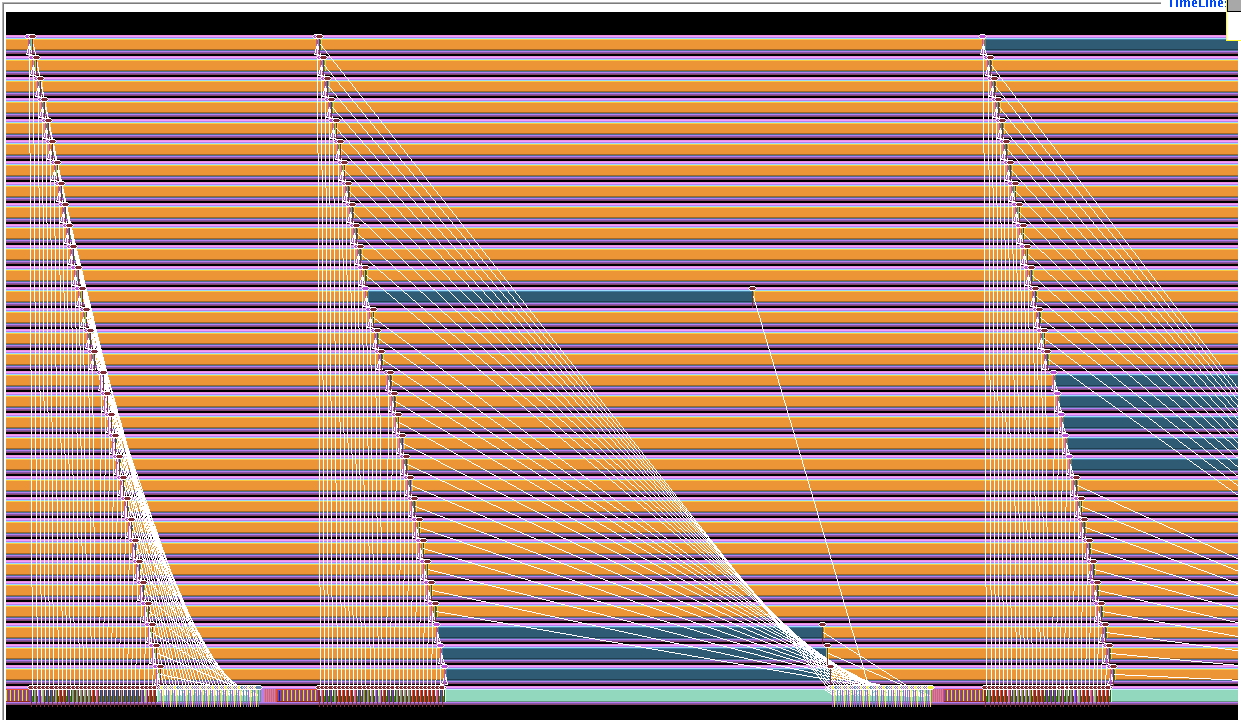
\includegraphics[scale=.35]{mandelbulk}
\caption{Trace of a bulk Mandelbrot calculation}
\label{fig:mandel-bulk}
\end{figure}

\Level 0 {Collective task scheduling}
\label{proj:mandel-collective}

Another implementation of the bulk scheduling of the previous section
would be through using collectives.

\begin{exercise}
  Code a solution which uses scatter to distribute data to the worker
  tasks, and gather to collect the results. Is this solution more or
  less efficient than the previous?
\end{exercise}

\Level 0 {Asynchronous task scheduling}

At the start of section~\ref{proj:mandel-bulk} we said that bulk scheduling
mostly makes sense if all tasks take similar time to complete.
In the Mandelbrot case this is clearly not the case.

\begin{exercise}
  Code a fully dynamic solution that uses \n{MPI_Probe} or \n{MPI_Waitany}.
  Make an execution trace and report on the total running time.
\end{exercise}

\begin{figure}[ht]
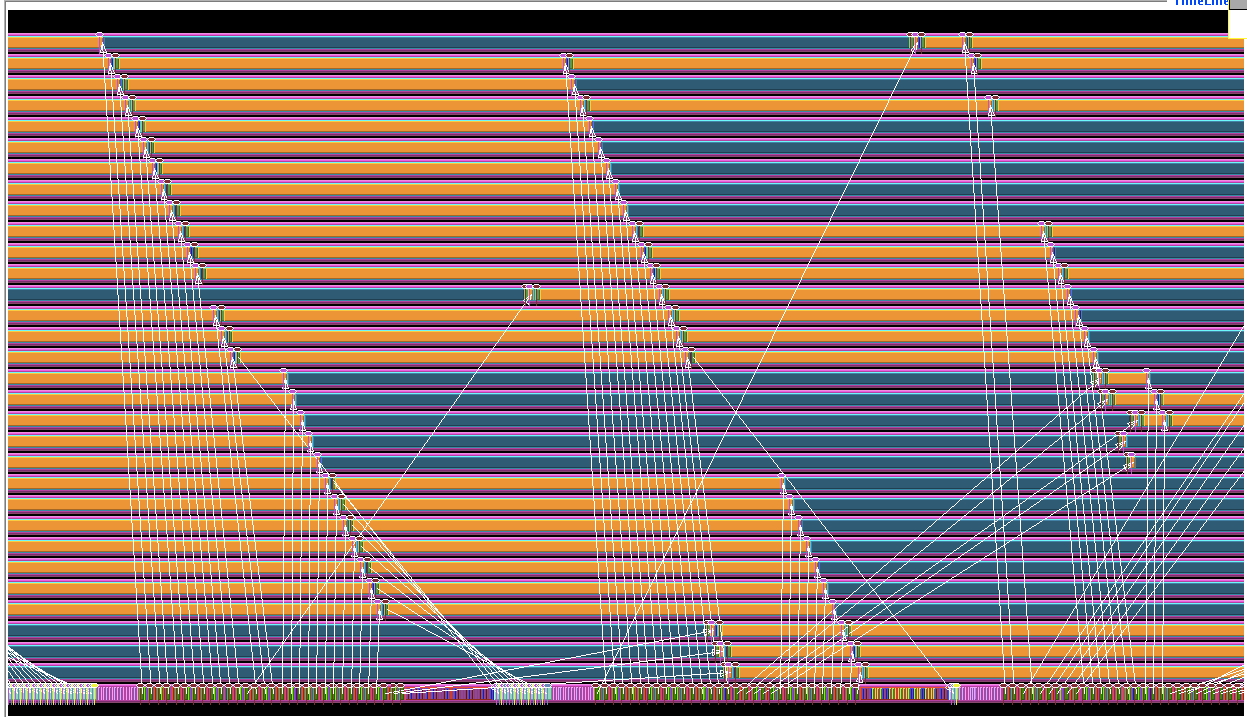
\includegraphics[scale=.35]{mandelasync}
\caption{Trace of an asynchronous Mandelbrot calculation}
\label{fig:mandel-async}
\end{figure}

\Level 0 {One-sided solution}

Let us reason about whether it is possible (or advisable) to code a
one-sided solution to computing the Mandelbrot set.  
%
With active
target synchronization you could have an exposure window on the host
to which the worker tasks would write. To prevent conflicts you would allocate an 
array and have each worker write to a separate location in it.
%
The problem here is that the workers may not be sufficiently synchronized because
of the differing time for computation.

Consider then passive target synchronization. Now the worker tasks could
write to the window on the manager whenever they have something to
report; by locking the window they prevent other tasks from interfering.
%
After a worker writes a result, it can get new data from an array
of all coordinates on the manager. 

It is hard to get results into the image as they become available. For
this, the manager would continuously have to scan the results
array. Therefore, constructing the image is easiest done when all
tasks are concluded.
